
\ifdefined\standalone 
\documentclass[12pt]{article}
\usepackage{graphicx}
\usepackage{float}
\usepackage[a4paper, margin=1in]{geometry}
\usepackage[utf8]{inputenc}
\usepackage{textcomp}
\usepackage{amsmath}
\usepackage{booktabs}
\usepackage{tikz}
\usepackage{enumitem}
\usetikzlibrary{decorations.pathmorphing,patterns}
\usepackage[hidelinks]{hyperref}

\begin{document}
\fi


\section{Instantaneous gas release rate}

This verification case evaluates the behaviour of the instantaneous gas release model.  
As shown in Figure~\ref{fig:instant_config}, a one-dimensional sample of thickness \(L = 10\ \mathrm{cm}\) is considered.  
A bottom gas influx of $\dot{m}^{''}_{\mathrm{g,ini}}= 0.1 \mathrm{kg\cdot m^{-2}\cdot s^{-1}}$ is imposed at the lower boundary.  
The sample undergoes controlled degradation that generates a constant volumetric production of volatile gases  
\(\dot{\omega}_{fg}^{'''} = 0.4\ \mathrm{kg\cdot m^{-3}\cdot s^{-1}}\) until complete consumption of the solid (at \(t = 1000\ \mathrm{s}\)). These conditions are obtained using the same reaction mechanism as in the verification case "Mixture Law"
\ifdefined\Verification
(Section \ref{sec:mixture-law}).
\else
.
\fi

Figures~\ref{fig:mlr_total} and \ref{fig:profile_flux} display respectively (i) the total mass flux and total mass loss rate,  
and (ii) the depth profile of the gas mass flux at \(t = 500\ \mathrm{s}\). The total mass flux corresponds to the sum of the intrinsic mass loss rate and the imposed inflow.  
Because the vertical axis in Gpyro is directed downward, upward gas motion appears as negative in sign.  

Since the gas production rate is constant throughout the domain, the analytical mass-flux distribution varies linearly: 


\begin{equation}
	\dot{m}^{''}_{\mathrm{gas}}(z) = -\dot{m}^{''}_{\mathrm{g,ini}}- \dot{\omega}_{fg}^{'''}(z - L)
\end{equation} 


A time step of \(1\ \mathrm{s}\) and spatial discretisation of \(\Delta z = 0.1\ \mathrm{mm}\) are used.

\begin{figure}[H]
\centering
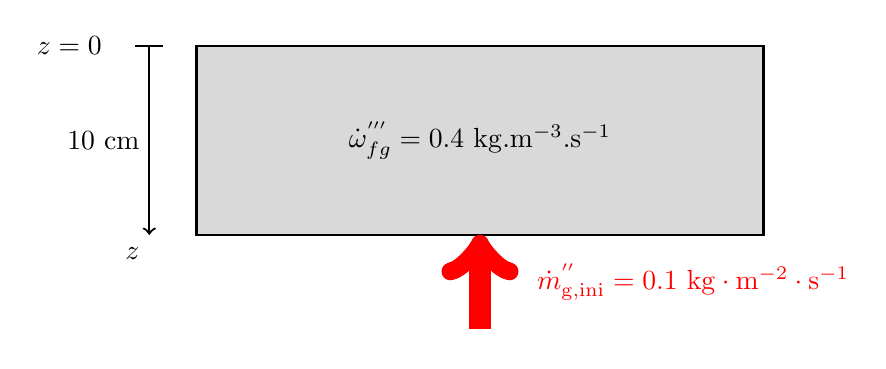
\begin{tikzpicture}[scale=1.2]

\draw[fill=gray!30,thick] (0,0) rectangle (6,2); 
\node at (3,1) {$\dot{\omega}_{fg}^{'''}=0.4 ~\mathrm{kg.m^{-3}.s^{-1}}$};

\draw[thick] (-0.35,2) -- (-0.65,2); 
\node[left] at (-0.9,2) {$z=0$};

\draw[thick,->] (-0.5,2) -- (-0.5,0);
\node[left] at (-0.5,1) {10~cm};
\node[left] at (-0.5,-0.2) {$z$};

\draw[red,line width=8pt,->] (3,-1) -- (3,0.0);
\node[red,anchor=west] at (3.5,-0.5)
    {$\dot{m}^{''}_{\mathrm{g,ini}} = 0.1~\mathrm{kg\cdot m^{-2}\cdot s^{-1}}$};

\end{tikzpicture}
\caption{Configuration schematic of the instantaneous gas-release test case.}
\label{fig:instant_config}
\end{figure}

\begin{figure}[H]
\centering

\begin{minipage}{0.48\textwidth}
\centering
\includegraphics[width=\linewidth]{Total_mass_flux_instantaneous.png}
\caption{Total mass flux and total mass loss rate.}
\label{fig:mlr_total}
\end{minipage}
\hfill
\begin{minipage}{0.48\textwidth}
\centering
\includegraphics[width=\linewidth]{profile_mass_flux_instantaneous.png}
\caption{Depth profile of mass flux at \(t=500\ \mathrm{s}\).}
\label{fig:profile_flux}
\end{minipage}

\end{figure}


\ifdefined\standalone
\end{document}
\fi



